The main goal of the thesis is the creation a tool that combines the algorithm estimates for LWE and SIS that we introduced above and can be configured without much knowledge of the workings of the underlying algorithms. To our knowledge there has not been a tool that includes the function of generically searching for secure parameters for both LWE and SIS instances as well as for ring and module variants. Some schemes (e.g. commitment schemes, see \cref{sec:two-problem-search}) depend on the statistical security of either LWE or SIS. We hence include classes respectively to find parameters satisfying this criteria. % TODO: maybe not here just in the section. 
Furthermore, we provide a set of utility classes and methods for most commonly used distributions and norms.
A configuration class allows for a substantial customization of the estimation process.
The tool can either estimate the bit security level of fixed parameter sets or generically search for parameter sets that satisfy a certain bit security level.

% class for distributions... from section this modelling, problems, generic search... Überblick, wie verwendbar,
% automatische norm umwandlung,
% sonstige features
\section{Supported Distributions} \label{sec:supported-distributions}% TODO
\subsection{Gaussian Distribution}
In some applications we receive a Gaussian distribution as input but require a bound in some norm in order to estimate the hardness of an SIS instance. Hence, we need to transform a Gaussian with parameter $s  = \sqrt{2 \pi} \sigma$ into a bound $\beta$ given some security parameter $sec$. Note that a $n$-dimensional Gaussian $D_{\mathbf{Z}^n, s}$ can be sampled by combining samples from $n$ independent one-dimensional Gaussians $D_{\mathbf{Z}, s}$ \cite{GJS15}. %TODO check

For a Gaussian distribution and a random variable $X$ with $X \sim D_{\mathbf{Z}, s}$, the following holds: % put as theorem, also for norm inequalities

\begin{equation}
    \text{Pr}\left[ |X| \geq \beta \right] \leq 2 e^{-\pi \|\mathbf{v}\|^2/s^2}
\end{equation}

We demand $2 e^{-\pi \beta^2/s^2} \approx 2^{-sec}$ with $\beta = \|\mathbf{v}\|$  and obtain

\begin{align*}
    2 e^{-\pi \beta^2/s^2}   & \approx 2^{-sec}                               \\
    -\pi \frac{\beta^2}{s^2} & \approx (-sec - 1)\ln (2)                      \\
    \beta                    & \approx s \sqrt{\frac{(sec + 1) \ln(2)}{\pi}}.
\end{align*}

\begin{theorem}[Gaussian to Bound]
    Given a Gaussian distribution $D_{\mathbf{Z}^n, s}$ with width parameter $s  = \sqrt{2 \pi} \sigma$ and a security parameter $sec$, we can compute a bound $\beta$ such that a sample $\mathbf{v}$ drawn from $D_{\mathbf{Z}^n, s}$ satisfies $\text{Pr}\left[ \|\mathbf{v}\| \geq \beta \right] \leq 2^{-sec}$ as follows:
    \begin{equation}
        \beta  \approx s \sqrt{\frac{(sec + 1) \ln(2)}{\pi}}.
    \end{equation}
\end{theorem}

The resulting bound $\beta$ is an $\ell_2$-norm bound. % TODO: distributions is changes => thanks Marc! (also noticed that it doesn't make sense to have componentwise and L2)


\subsection{Uniform Distribution}
The secret distribution 



\section{Norms and Bounds} % TODO: check
%TODO: write some prose about why we need that
% TODO: make sure that it is clear that these are bounds!!!
Let $\mathcal{R}_q$ be a ring as defined in \cite{BDLOP18} and $f \in \mathcal{R}_q$ with $f = \sum_i f_i X^i$. Following \cite{BDLOP18} we define the norms
\begin{align}
    \ell_1 : \| f| \|_1           & = \sum_i |f_i|,                                           \\
    \ell_2 : \| f| \|_2           & = \left(\sum_i |f_i|^2\right) ^{\frac{1}{2}}, \text{ and} \\
    \ell_\infty : \| f| \|_\infty & = \max_i |f_i|.
\end{align}

Then the following inequations hold \cite{BDLOP18}:
\begin{align}
    \| f \|_1      & \leq \sqrt{n} \| f \|_2 \label{norm1}                                                                    \\
    \| f \|_1      & \leq n \| f \|_\infty \label{norm2}                                                                      \\
    \| f \|_2      & \leq \sqrt{n} \| f \|_\infty \;\;(\text{since }  \sqrt{n} \| f \|_2 \leq n \| f \|_\infty) \label{norm3} \\
    \| f \|_\infty & \leq \| f \|_1 \label{norm4}
\end{align}

Let $\mathcal{O}_K$ be the ring of integers of a number field $K=\mathbb{Q}(\theta)$, where $\theta$ is an algebraic number and $\sigma$ denote the canonical embedding as defined in \cite{DPSZ12}. Then, following \cite{DPSZ12} for $f \in \mathcal{O}_K$ it holds the following inequations hold (we assume that $C_m = 1$): % TODO: why?
\begin{align}
    \| f \|_\infty         & \leq \| \sigma(f) \|_\infty \label{norm5}, \\
    \| \sigma(f) \|_\infty & \leq \| f \|_1 \label{norm6}.
\end{align}

From the above inequations, we obtain the following theorems.
\begin{theorem}[Relationships Between Norm Bounds \cite{BDLOP18,DPSZ12}]\label{th:norm-rel}
    Given a ring element $f \in \mathcal{O}_K$ as defined above, then we can bound norms by $\ell_p$-norms as follows:
    \begin{itemize}
        \item From \cref{norm1}, it follows that $\| f \|_1 \leq \sqrt{n} \| f \|_2$ and from \cref{norm2}, $\| f \|_1 \leq n \| f \|_\infty$.
        \item From \cref{norm3} and \cref{norm4}, it follows that $\| f \|_2 \leq \sqrt{n}  \| f \|_1$ and from \cref{norm3}, $\| f \|_2 \leq \sqrt{n}  \| f \|_\infty$.
        \item From \cref{norm4}, it follows that $\| f \|_\infty \leq  \| f \|_1$ and from \cref{norm1} and \cref{norm4}, $\| f \|_\infty \leq \sqrt{n}  \| f \|_2$.
        \item From \cref{norm6}, it follows that $\| \sigma(f) \|_\infty \leq  \| f \|_1$, from \cref{norm1} and \cref{norm6}, $\| \sigma(f) \|_\infty \leq \sqrt{n}  \| f \|_2$, and from \cref{norm2} and \cref{norm6}, $\| \sigma(f) \|_\infty \leq n  \| f \|_\infty$.
    \end{itemize}
    Likewise, we get the following bounds for the $\mathcal{C}_\infty$-norm:
    \begin{itemize}
        \item From \cref{norm2} and \cref{norm5}, it follows that $\| f \|_1 \leq  n \| \sigma(f) \|_\infty$.
        \item From \cref{norm3} and \cref{norm5}, it follows that $\| f \|_2 \leq  \sqrt{n} \| \sigma(f) \|_\infty$.
        \item From \cref{norm5}, it follows that $\| f \|_\infty \leq  \| \sigma(f) \|_\infty$.
    \end{itemize}
\end{theorem}

We also want to be able to add and multiply bounds from different norms. Note that the degree of the polynomial of the underlying ring to which we apply the norms must match. To add two bounds we simply bound the second addend by the used norm of the first as described in \cref{th:norm-rel} and add both bounds to obtain a bound in the norm of the first addend. It is slightly more complicated for multiplication and we state the results in the next theorem.

\begin{theorem}[Multiplication of Norm Bounds \cite{BDLOP18, DPSZ12}]
    Let $f$ be defined as above and let $g \in \mathcal{R}_q$ where $g = \sum_i \overline{g}_i X^i$ where $g_i \in \left[-(q-1)/2, (q-1)/2\right]$ and $\overline{g}_i = g_i \mod q$ as in \cite{BDLOP18}. We then can define the following inequations for multiplication according to \cite{BDLOP18}:

    \begin{itemize}
        \item If $\|f\|_\infty \leq \beta, \|g\|_1 \leq \gamma$ then $\|f \cdot g\|_\infty \leq \beta \cdot \gamma$.
        \item If $\|f\|_2 \leq \beta, \|g\|_2 \leq \gamma$ then $\|f \cdot g\|_\infty \leq \beta \cdot \gamma$.
    \end{itemize}

    Let $x, y \in \mathcal{O}_K$. Again, we assume that $C_m = 1$. Then, the following inequation holds according to \cite{DPSZ12}:
    \begin{align}
        \| x \cdot y \|_\infty \leq C_m \cdot n^2 \cdot \| x \|_\infty \cdot \| y \|_\infty \\
        \| \sigma(x \cdot y) \|_\infty \leq  \| \sigma(x) \|_\infty \cdot \| \sigma(y) \|_\infty.
    \end{align}
\end{theorem}




\section{Problem Classes}
We now present the problem classes in $\texttt{lattice\_parameter\_estimation/problem}$ (see \cref{fig:problem-classes}).

\begin{figure}[h]
    \centering
    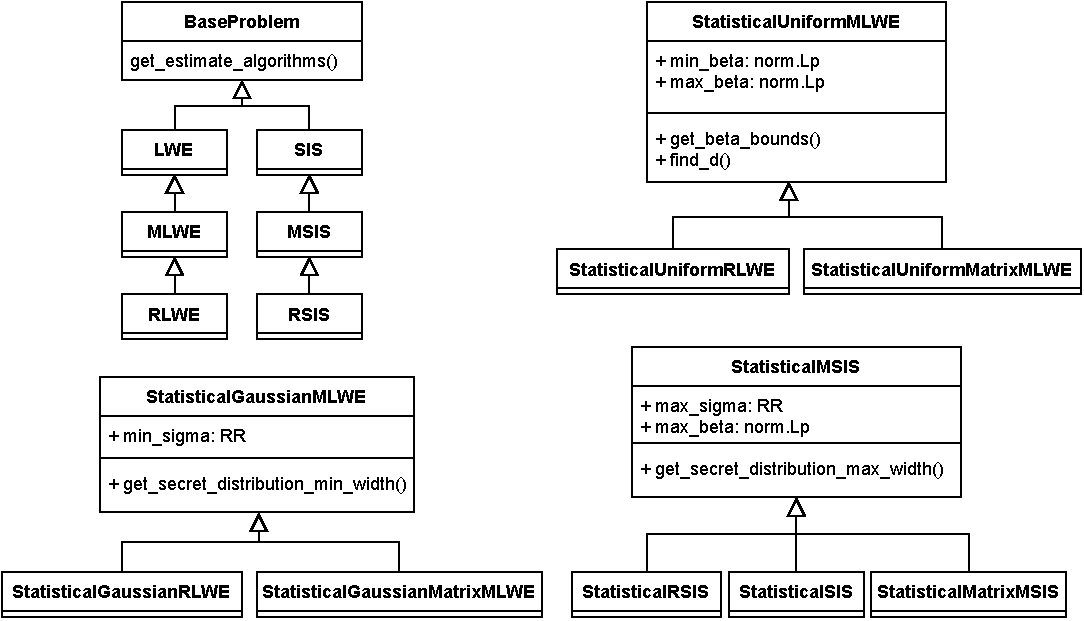
\includegraphics[width=1\textwidth]{graphics/problem_classes.pdf}
    \caption{Problem Classes}\label{fig:problem-classes}
\end{figure}

$\texttt{LWE}$ and $\texttt{SIS}$ inherit from the base class $\texttt{BaseProblem}$ respectively. All instances provide a method $\texttt{get\_estimate\_algorithms()}$ that returns a list of algorithm instances that can be executed by the function $\texttt{estimate()}$. Furthermore, any instance of $\texttt{BaseProblem}$ can be compared to a bit security level (for more details, we refer the reader to the documentation). The $\texttt{LWE}$ class is initialized by the secret dimension $n$, a modulus $q$, the number of samples $m$, a $\texttt{secret\_distribution}$ and a $\texttt{error\_distribution}$. Both $\texttt{secret\_distribution}$ and $\texttt{error\_distribution}$ must be instances of the class $\texttt{distributions.Distribution}$. Instead of $\texttt{secret\_distribution}$ and $\texttt{error\_distribution}$, a bound of type $\texttt{norm.BaseNorm}$ must be set for $\texttt{SIS}$. Note that both {distributions.Uniform} and {distributions.Gaussian} are instances of $\texttt{norm.BaseNorm}$ and can thus be used as a bound. We compute the bound for a given distribution instance as described in \cref{sec:supported-distributions}.

For ring and module variants $\texttt{RLWE}$, $\texttt{RSIS}$ and $\texttt{MLWE}$, $\texttt{MSIS}$ respectively $n$ denotes the degree of the polynomial of the underlying ring $\mathcal{R}_q$. The module variants $\texttt{MLWE}$ and $\texttt{MSIS}$ take an addition parameter $d$ for the rank of the module.

While there exist special cases where the ring structure of problem instances can be exploited in an attack on LWE or SIS, % TODO: find examples
in general, the hardness of ring and Module variants is estimated by interpreting the coefficients of elements of $\mathcal{R}_q$ as vectors in $\mathbb{Z}_q^n$ \cite{ACDDPPVW18}.
We thus reduce ring and Module instances as follows when calling $\texttt{get\_estimate\_algorithms()}$ on the ring and module variant of $\texttt{LWE}$ and $\texttt{SIS}$:
\begin{itemize}
    \item RLWE$_{n, q, m, \chi} \longrightarrow$ LWE$_{n, q, m \cdot n, \chi}$
    \item MLWE$_{n, d, q, m, \chi} \longrightarrow$ LWE$_{n \cdot d, q, m \cdot n, \chi}$
    \item RSIS$_{n, q, m, \beta} \longrightarrow$ SIS$_{n, q, m \cdot n, \beta}$
    \item MSIS$_{n, d, q, m, \beta} \longrightarrow$ SIS$_{n \cdot d, q, m \cdot n, \beta}$
\end{itemize}


\paragraph{$\texttt{StatisticalGaussianMLWE}$.} For LWE, we define a statistically secure variant over a Gaussian distribution and over a uniform distribution. $\texttt{StatisticalGaussianMLWE}$ follows Corollary 7.5 and Theorem 7.4 in \cite{LPR13}. To avoid confusion we first specify the mapping for differing usage of parameters in \cite{LPR13} as compared to this work \cref{tab:mapping-LPR13} and obtain the following theorem:

\begin{table}
    \centering
    \begin{tabular}[h]{lll}
        \toprule
        Parameters in \cite{LPR13} & Use Here & Represents                    \\\hline
        $l$                        & $m+d$    & width of matrix $\mathbf{A}$  \\
        $k$                        & $m$      & height of matrix $\mathbf{A}$ \\
        \bottomrule
    \end{tabular}
    \caption{Parameter Mapping from \cite{LPR13}}\label{tab:mapping-LPR13}
\end{table}

\begin{theorem}{Statistically Secure MLWE Over a Gaussian Distribution \cite{LPR13}}
    Let $\mathcal{R}$ be the ring of integers in the $m'$th cyclotomic number field $K$ of degree $n$, and $q \geq 2$ an integer.
    For positive integers $m \leq m + d \leq \text{poly}(n)$, let $\mathbf{A} = [ \mathbf{I}_{[m]} \mid \bar{\mathbf{A}}] \in (\mathcal{R}_q)^{[m] \times [m+d]}$, where $\mathbf{I}_{[m]} \in (\mathcal{R}_q)^{[m] \times [m]}$ is the identity matrix and $\bar{\mathbf{A}} \in (\mathcal{R}_q)^{[m] \times [d]}$ is uniformly random.
    Then with probability $1 - 2^{-\Omega(n)}$ over the choice of $\bar{\mathbf{A}}$, the distribution of $\mathbf{A}\mathbf{x} \in (\mathcal{R}_q)^{[m]}$ where each coordinate of $\mathbf{x} \in (\mathcal{R}_q)^{[m+d]}$ is chosen from a discrete Gaussian distribution of parameter $s > 2n \cdot q^{m / (m+d) + 2/(n (m+d))}$ over $\mathcal{R}$, satisfies that the probability of each of the $q^{n m}$ possible outcomes is in the interval $(1 \pm 2^{-\Omega(n)}) q^{-n }$ (and in particular is within statistical distance $2^{-\Omega(n)}$ of the uniform distribution over $(\mathcal{R}_q)^{[m]}$). % TODO change [x]times[y] notation???
\end{theorem}
% TODO: anything more? can you provide an intuition?

If a security parameter is passed and $sec > n$, we raise an exepction.
The resulting minimal standard deviation is stored in the instance variable $\texttt{min\_sigma}$ and the corresponding distribution can be obtained by calling $\texttt{get\_secret\_distribution\_min\_width()}$ on the class instance.



\paragraph{$\texttt{StatisticalUniformMLWE}$.} The authors of \cite{BDLOP18} describe statistically secure MLWE instances over a Uniform distribution with invertible elements. The samples $(\mathbf{A}', h_{\mathbf{A}'}(y))$ of the resulting MLWE instance are within statistical distance $2^{-sec}$ of $(\mathbf{A}', \mathbf{u})$ for uniformly distributed $\mathbf{u}$. % TODO: check formulation

In \cref{tab:mapping-BDLOP18} we specify the mapping of parameters used in \cite{BDLOP18} and obtain the following theorem: %TODO 

\begin{table}
    \centering
    \begin{tabular}[h]{lll}
        \toprule
        Parameters in \cite{BDLOP18} & Use Here & Represents                                         \\\hline
        $k$                          & $m+d$    & width of matrix $[ \mathbf{I}_n \; \mathbf{A}' ]$  \\
        $n$                          & $m$      & height of matrix $[ \mathbf{I}_n \; \mathbf{A}' ]$ \\
        $d$                          & $d_2$    & variable                                           \\
        $N$                          & $n$      & degree of Ring polynomial                          \\
        \bottomrule
    \end{tabular}
    \caption{Parameter Mapping from \cite{BDLOP18}}\label{tab:mapping-BDLOP18}
\end{table}


\begin{theorem}[Statistically Secure MLWE Over a Uniform Distribution \cite{BDLOP18}]
    Let $1 < d_2 < n$ be a power of 2. If $q$ is a prime congruent to $2d_2 + 1 \;(\text{mod } 4d_2)$ and
    \begin{equation}
        q^{m/(m+d)} \cdot 2^{2 sec/((m+d)\cdot n)} \leq 2 \beta < \frac{1}{\sqrt{d_2}} \cdot q^{1/d_2}
    \end{equation}
    then any (all-powerful) algorithm $\mathcal{A}$ has advantage at most $2^{-sec}$ in solving $\text{DKS}_{m,m+d,\beta}^\infty$, where $\text{DKS}^\infty$ is the decisional knapsack problem in $\ell_\infty$-norm.
\end{theorem}


Hence, we have:
\begin{align}
    \beta_{min} & = \frac{q^{m/(m+d)} \cdot 2^{2 sec/((m+d)\cdot n)}}{2} \\
    \beta_{max} & = \frac{1}{2\sqrt{d_2}} \cdot q^{1/d_2} - 1
\end{align}
% TODO: explain ho to arrive at 2*sec instead of 256 

The variable $d_2$ can be passed as an argument. If it is not passed, we try to find $d_2$ by iterating over all powers of $2$ that are smaller than $n$.
The resulting bounds are converted to $\ell_\infty$ and stored in the instance variables $\texttt{min\_beta}$ and $\texttt{max\_beta}$. We also provide an instance method $\texttt{get\_beta\_bounds()}$ to obtain a tuple of both.

For both statistically secure MLWE variants, we include the corresponding ring versions $\texttt{StatisticalGaussianRLWE}$ and $\texttt{StatisticalUniformRLWE}$ for $d=1$ and matrix versions $\texttt{StatisticalGaussianMatrixMLWE}$ and $\texttt{StatisticalUniformMatrixMLWE}$ for which the width and height of the matrix $\mathbf{A}$ in \cite{LPR13} can be passed instead of $m$ and $d$. % TODO: include instead of included?
% TODO: explain why this doesn't work for LWE


\paragraph{$\texttt{StatisticalMSIS}$.} We can find parameters for a statistically secure MSIS instance by following Section 4.1 of \cite{DOTT21}. More specifically, we ask to find a MLWE instance where the probability that non zero elements $\mathbf{r}$ in the Euclidean ball $B_{m}(0, 2B)$ satisfy $\hat{\mathbf{A}}_1 \cdot \mathbf{r} = \mathbf{0}$ is smaller than $2^{-sec}$. % TODO check that this is not a quote

We give a mapping of the parameters in \cite{DOTT21} in \cref{tab:mapping-DOTT21}

\begin{table}
    \centering
    \begin{tabular}[h]{lll}
        \toprule
        Parameters in \cite{DOTT21} & Use Here & Represents                            \\\hline
        $m'$                        & $m+d$    & width of matrix $\hat{\mathbf{A}}_1$  \\
        $m$                         & $m$      & height of matrix $\hat{\mathbf{A}}_1$ \\
        $B$                         & $B$      & norm-bound of secret                  \\
        $s$                         & $s$      & Gaussian width (not stddev)           \\
        $N$                         & $n$      & degree of polynomial                  \\
        \bottomrule
    \end{tabular}
    \caption{Parameter Mapping from \cite{DOTT21}}\label{tab:mapping-DOTT21}
\end{table}


The number of elements in $B_{m+d}(0, 2B)$ can be estimated from above as $|B_{m+d}(0, 2B)| \ll (2 \pi e /((m+d) n))^{(m+d) n/2} \cdot (2 B)^{(m+d) n}$. The scheme is statistically binding if the probability that non zero elements in $B_{m+d}(0, 2B)$ of radius $2B$ in $\mathcal{R}_q^{m+d}$ map to $\mathbf{0}$ in $\mathcal{R}_q^{m}$ is negligible. Hence, it must hold that $|B_{m+d}(0, 2B)|/q^{m n} \leq 2^{-sec}$ and we get:

% TODO: look for bound of ball without o(...) if change also change in docstring

\begin{align}
    \left(\sqrt{\frac{2 \pi e}{(m+d) \cdot n}} \cdot 2 B\right)^{(m+d) \cdot n} & \leq 2^{-sec} \cdot q^{m\cdot n}                                                                       \\
    B                                                                           & \leq 2^{\frac{-sec}{(m+d)\cdot n} - 1} \cdot q^\frac{m}{m+d} \cdot \sqrt{\frac{(m+d)\cdot n}{2 \pi e}}
\end{align}

We convert the bound $B$ to a Gaussian over $\ell_2$-norm by following the procedure described in \cref{sec:norm}: % TODO: add appropriate reference

\begin{equation}
    s  \approx x \sqrt{\frac{\pi}{(sec + 1) \ln(2)}}
\end{equation}

% TODO: rephrase to obtain a lemma?
The resulting parameters $B$ and $s$ can be accessed by the instance variables $\texttt{max\_sigma}$ and $\texttt{max\_beta}$ or by calling $\texttt{get\_secret\_distribution\_max\_width()}$ on the class instance.

As for statistically secure MLWE we again include a matrix version $\texttt{StatisticalMatrixMSIS}$ and a ring $\texttt{StatisticalRSIS}$ by setting $d=1$. In addition, the proof also applies to the base SIS variant and hence we include $\texttt{StatisticalSIS}$. Here the height of the matrix $n$ becomes the rank of the modulus in the MSIS instance, i.e. $d=n$, and the degree of the polynomial is $1$.




\section{Parameter Search and Configuration Options}
We now describe the main parameter search and estimate configuration options in our tool. The configuration can be customized by using the class $\texttt{algorithms.Configuration}$ and passed as an optional argument of $\texttt{param\_search.generic\_search()}$. It is also possible to directly estimate the cost of a list of parameter problems by calling the function $\texttt{problem.estimate()}$. For more details we again refer to the documentation.

\paragraph{Cost Models.} Attacks that use BKZ for lattice reduction require a cost model to estimate the number of CPU cycles in the SVP subroutine. Default cost models are shown in \cref{tab:costmodels}. We distinguish between estimates for classical, quantum, sieving and enumeration and each of these categories can be deselected by setting the respective parameter to $\texttt{False}$. Note that at least one of classical and quantum and of sieving and enumeration respectively must be selected to make use of the default cost models. If all are unselected custom cost models must be specified and passed as an argument. We included an option of taking the most conservative estimate for each category combination for a more efficient parameter search or estimation. Furthermore, we assigned a priority value on an ordinal scale to each cost model which enables us to first run cost models that yield a lower cost and thus terminate the estimation process earlier for an insecure parameter set. The priority values of the default cost models are derived from \cref{fig:costmodels}.
\begin{figure}[h]
    \centering
    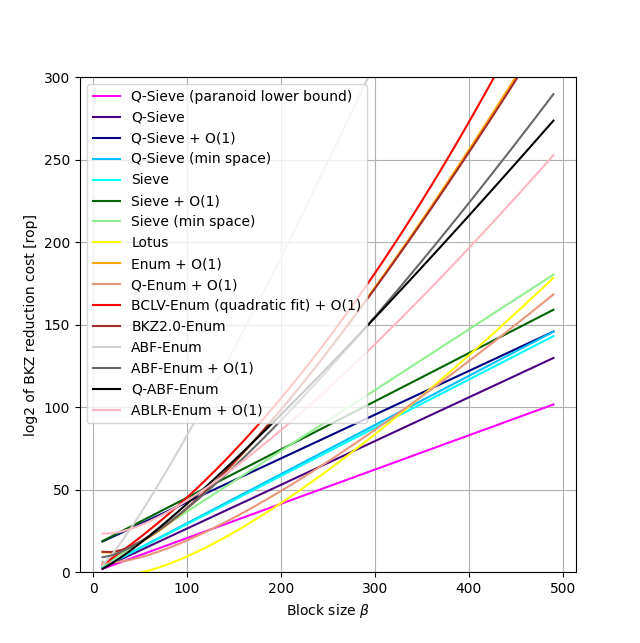
\includegraphics[width=0.7\textwidth]{graphics/cost_models.png}
    \caption{Cost Models}\label{fig:costmodels}
\end{figure}
The number of BKZ rounds can be configured by passing a function with parameters $\texttt{beta, d}$ where $\texttt{beta}$ is the block size and $\texttt{d}$ the lattice dimension. In the default configuration we use the more conservative ``Core''-SVP model $\texttt{algorithms.BKZ\_SVP\_repeat\_core}$ \cite{ADPS16} in which the polynomial factor of the runtime complexity of BKZ is completely ignored. In addition, we provide a model $\texttt{algorithms.BKZ\_SVP\_repeat\_8d}$ for a BKZ cost of $8 \cdot d \cdot t_k$ BKZ rounds where $d$ again referes to the lattice dimension (see \cref{sec:bkz-8d}).


\subsection{Generic Search and Estimate Algorithms}
The main functionality of our tool is encapsulated in the function $\texttt{param\_search.generic\_search()}$. The high-level idea of the search is presented in \cref{alg:generic-search}. We begin with an initial parameter set. We then create a list of problem instances generated by a $\texttt{parameter\_problem}$ function and estimate the cost of all instances in the list. If the list contains multiple SIS instances or multiple LWE instances, we attempt to reduce the instances to the easiest problem instance respectively. % TODO: include how, \cref{sec:problem-reduction} 
Once the $\texttt{estimate}$ function finds an instance that is insecure (i.e. the estimated attack cost in clock cycles is smaller than $2^{sec}$), it terminates the estimation procedure and returns an insecure result. We then use the $\texttt{next\_parameters}$ function to generate a list L of (multiple) new parameter sets from our current parameter set and sort each of the new parameter sets into an ordered list (duplicates are not accepted). The order is defined by a $\texttt{parameter\_cost}$ function. In the next step we retrieve the parameter set with the lowest cost from L and repeat the procedure until the cost estimation step returns a secure result. The result includes the estimates for all cost models and algorithms.

\begin{algorithm2e} % TODO: check if block is not of dimension kxk
    \SetKwBlock{Begin}{function}{end function}
    \Begin(generic\_search(sec, initial\_params, next\_parameters, parameter\_cost,  problem\_instance)) % TODO nxn???
    {
        L = OrderedList(initial\_params)\\
        \While{L $\neq \emptyset$}{
            current\_params = L.pop() \\
            instances = parameter\_problem(current\_params) \\
            result = estimate(instances, sec) \\
            \If{result is secure}{
                Return result\\
            }
            \Else{
                next\_param\_sets = next\_parameters(current\_params)\\
                \ForAll{param\_set in next\_param\_sets}{
                    sort param\_set into L according to parameter\_cost function\\
                }
            }
        }

    }
    \caption{Generic Search} \label{alg:generic-search}
\end{algorithm2e}

The $\texttt{estimate}$ function can be configured to run in parallel in the configuration which may speed up the search, in particular if many cost models need to be tested (e.g. with configuration setting $\texttt{conservative=False}$ and long running algorithms like $\texttt{ARORA\_GB}$, $\texttt{CODED\_BKW}$ and $\texttt{PRIMAL\_DECODE}$ are used. The list of used algorithms can be changed in the configuration. We recommend to include $\texttt{PRIMAL\_USVP}$ for LWE instances and $\texttt{LATTICE\_REDUCTION}$ for SIS instances to make full use of early termination since the estimate algorithms for these attacks have a short runtime and yield relatively low cost estimates.


\cref{fig:SIS-algs}, \ref{fig:LWE-algs-small} and \ref{fig:LWE-algs-large} show the plots of runtime and performance tests for the various algorithms that can be used in our tool. In accordance with the results, we assigned priority values on an ordinal scale to the estimation algorithms. In \cref{tab:lwe-alg-prio} and \ref{tab:sis-alg-prio} we present the list of algorithms and their corresponding priority values and justify our choice. Algorithms with a smaller priority are expected to yield relatively good results quickly and can therefore be executed first. If the estimate result does not satisfy the specified security requirement we can terminate the estimation process early in order to maximize the efficiency of our search.

\begin{figure}[]
    \centering
    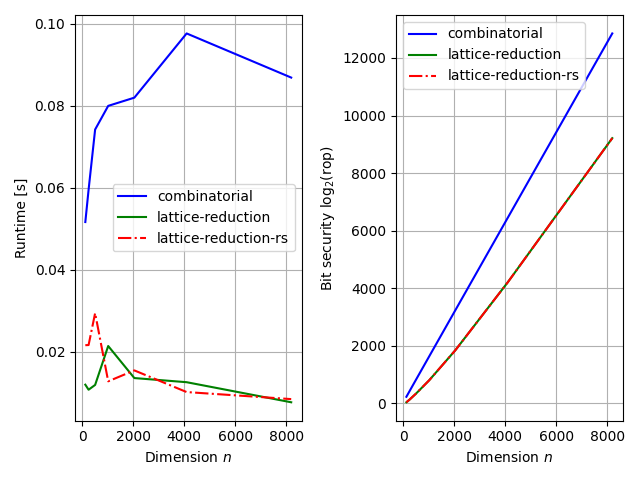
\includegraphics[width=0.8\textwidth]{graphics/SIS_stddev=2,828_plots_1s.png}
    \caption{SIS instance with $\sigma=2.828,\; m=n^2, \; 2^{2n} < q < 2^{2n+1}$}\label{fig:SIS-algs}
\end{figure}

\begin{figure}[]
    \centering
    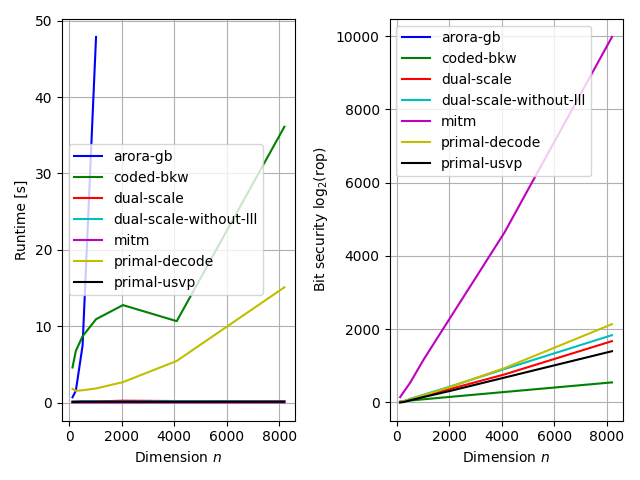
\includegraphics[width=0.8\textwidth]{graphics/LWE_stddev=0,125_plots_200s.png}
    \caption{LWE instance with $\sigma=0.125,\; m=\infty, \; 2^{n} < q < 2^{n+1}$}\label{fig:LWE-algs-small}
\end{figure}

\begin{figure}[]
    \centering
    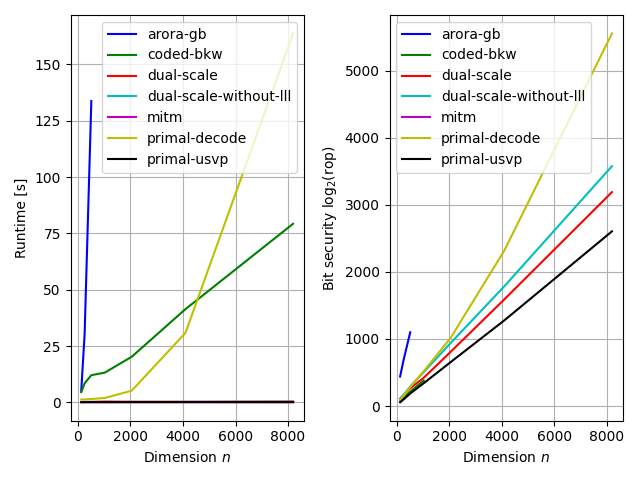
\includegraphics[width=0.8\textwidth]{graphics/LWE_stddev=2,828_plots_200s.png}
    \caption{LWE instance with $\sigma=2.828,\; m=\infty, \; 2^{n} < q < 2^{n+1}$}\label{fig:LWE-algs-large}
\end{figure}

% TODO: how does dual attack without LLL work???
\begin{table}
    \centering
    \begin{tabular}[]{lll}
        \toprule
        Algorithm                 & Priority & Justification                                       \\\hline
        Meet-in-the-Middle        & 5        & fastest, high cost estimate, as prefilter           \\
        Primal-uSVP               & 10       & fast, low cost estimatate estimates                 \\
        Dual Attack               & 20       & fast, often higher estimates than primal-usvp       \\
        Dual Attack (without LLL) & 30       & fast, often higher estimates than dual              \\
        Coded-BKW                 & 90       & slow, somtimes very low cost estimate               \\
                                  &          & (for small stddev), does not always yield results   \\
        Decoding Attack           & 100      & slow, often higher estimates than faster algorithms \\
        Arora-Ge                  & 200      & extremely slow, often higher estimates,             \\
                                  &          & does not always yield results                       \\
        \bottomrule
    \end{tabular}
    \caption{LWE Estimate Algorithm Priorities}\label{tab:lwe-alg-prio}
    \vspace{1cm}
    \begin{tabular}[]{lll}
        \toprule
        Algorithm                     & Priority & Justification                            \\\hline
        Lattice Reduction \cite{MR09} & 5        & fastest, low cost estimates              \\
        Lattice Reduction \cite{RS10} & 7        & same results as lattice-reduction,       \\
                                      &          & not always applicable                    \\
        Combinatorial Attack          & 10       & fast, often slightly higher cost results \\
        \bottomrule
    \end{tabular}
    \caption{SIS Estimate Algorithm Priorities}\label{tab:sis-alg-prio}
\end{table}

% TODO first finish section on algorithms
% - include plots
% - write about pro/cons
% - maybe add section of cost comparison for the algorithms of the previous section
